\chapter{Introduction}
\label{chapter_1_intro}
\graphicspath{ {./chapter-sp/figures/} }
\captionsetup[figure]{labelfont=bf}
\captionsetup{margin=1.5em}
\captionsetup[table]{labelfont=bf}


%%Definition of optical design
Optical design, generally speaking, can refer to the activities that manipulate light to achieve a certain purpose. This can be designing a telescope to observe remote celestial bodies, designing a concentrator to maximally harvest the solar energy, or designing optical fibre to maximize efficiency for information transmission. In the community of optical engineering, optical design is commonly associated with optical lens design. That means using optical lenses as the manipulator of light. The focus of this dissertation will also be the design of optical lenses. However, the insights summarized in this dissertation can also be extended to the design with other optical manipulators (e.g. mirrors).

In lens design, the light is usually modeled with its geometrical model(or ray model). The light propagation is described in terms of light rays. When the wavelength of the light is very small compared to the size of the structures with which light interacts, it is an excellent approximation. That also indicates the wave property of light such as interference and diffraction, is not captured by the geometrical model. The utilization of the simpler geometric model is mostly driven by the practicality of optical design: with geometrical optics where light is simplified as rays pointing towards the traveling direction of radiation energy, billion of rays can be traced in seconds for a standard modern personal computer. The performance of the system can be quickly determined for subsequent analysis or optimization. On the other side, with the more rigorous wave model, designing and analyzing a common optical system is computationally expensive, hence very time consuming and inconvenient to rapidly compute and optimize the system performance. 

%(reserved descriptions) However, conventionally, it usually means designing optical systems where light is mainly treated with its geometrical model rather than its more complicated wave model. These optical systems can be a photographic camera, a lamp or a laser beam-shaper, etc.. The aperture sizes of these optical systems are normally from several millimeters to meters. They are very large compared to the operating wavelength of the systems. Therefore, it is safe to apply the geometrical model and it maintains the essence of light that is sufficient to obtain a reasonable optical system design.

%what I want to emphazie is the use of both models, but the description is not well polished.
 % wave model: diffraction limited field analysis - diffraction, interference analysis (highly coherent beams), polarization
 
In some occasions, a wave model is necessary to be applied to understand the system performance. For instance, when an imaging system is only limited by diffraction, analyzing the intensity distribution of a focused beam at the focal plane requires a wave model. A geometrical model will only predict an extreme small spot without the information about the intensity distribution. As a result, depending on the performance requirements, practice for optical system design may involve both geometrical and wave models. A geometrical model is usually used to rapidly obtain a system solution that is good enough in terms of its performance predicted by the geometrical model. When approximation with the geometrical model is no longer accurate, the wave model helps to provide further analysis which gives feedback to fine-tune the system performance. The later part is usually involved in systems with a demanding performance requirement such as microscopic objectives or photo-lithographic projection systems. In this dissertation, the discussion is focused on designing optical systems based on the principles of geometrical optics. The wave model related analysis is not in scope.  


In geometrical optics, one of most important laws would be the law of refraction (also know as the Snell's law). It describes how a light ray travels at the interface of two different media:
\begin{equation}
n \sin i = n^\prime \sin r,
\label{eq: snellslaw}
\end{equation}
where $n$ and $n^\prime$ are the refractive indices of the media before and after refraction of a ray; $i$ and $r$ are the angles of the incidence and refraction at the interface between the two media. According to the law of refraction, lenses are designed to manipulate the light.
\begin{figure}
    \centering
    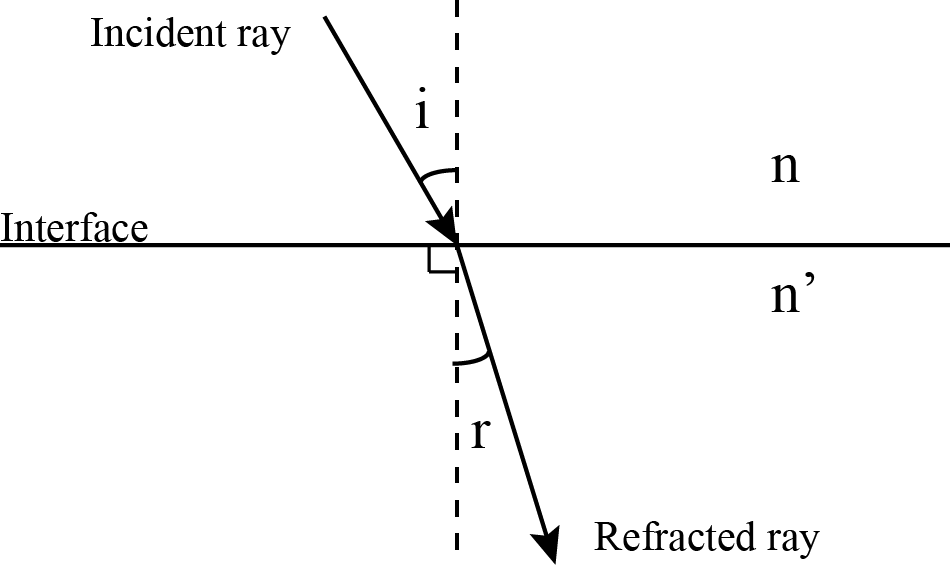
\includegraphics[scale=0.65]{chapter-1/figures/snellslaw.png}
    \caption{Snell's law: the light ray is refracted at the interface between the two media. The relation between the incident ray and the refracted ray is given by Equation \ref{eq: snellslaw}.}
    \label{fig: snellslaw}
\end{figure} 

The earliest known lenses were made by the ancient Egyptians and Mesopotamians \cite{wiki:HistoryofOptics}. They were made from polished crystal, often quartz, and are dated as early as 750BC for Assyrian lenses such as the Nimrud/Layard lens \cite{wiki:Nimrudlens}. The exact function of these lenses is not clear, with some authors suggesting that they were used as an optical lens (magnifying glasses) and others suggesting a decorative function. These lenses were mainly made by trial and error where actual understanding of the light was very limited. When people had more knowledge about geometrical optics, optical design started to pay attention to how light rays travel. With the increasing understanding of the nature of light, the design of optics also evolved from simple lenses to complicated systems which can achieve resolutions down to nanometers. This can not be achieved without the development of modern computer-aided optical design with which the performance of the optical system can be rapidly estimated and numerical optimization can be applied to further improve the system performance.

% background of the lens design approach
In modern optical lens design, an optical system is parameterized in design software. The designer studies the design requirements and determines what the initial configuration of the optical lens should be. Figure \ref{fig:chap0 model design flow} provides a flowchart of a modern optical design process. The optical designer then needs to start modifying the system based on his/her knowledge and observation with a purpose of meeting the design requirements. Numerical optimization, which is widely used in the computer-aid design, is also heavily applied in this step for lens design. With the help of the optimizer, the designer "guides" the system towards a desired configuration. 

\begin{figure}
    \centering
    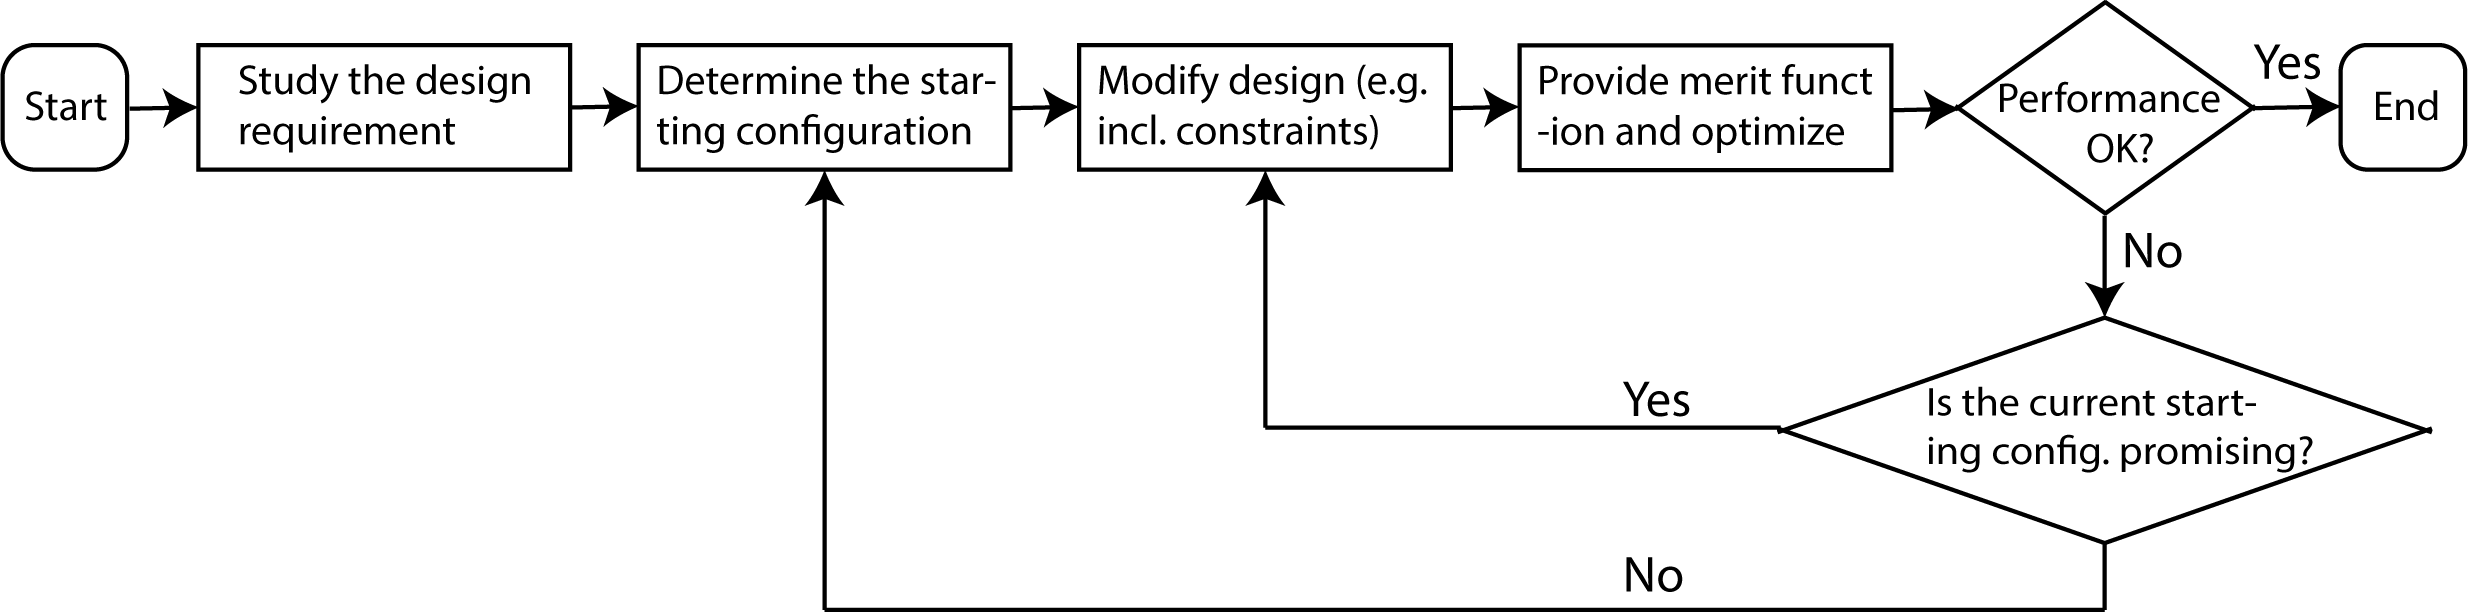
\includegraphics[scale=0.58]{chapter-0/figures/lens_design_flow_chart.png}
    \caption{Flowchart of the modern optical design process.}
    \label{fig:chap0 model design flow}
\end{figure} 

It is now understood and observed that the high-dimensional design (optimization) space formed by the variables of the parameterized optical system are nonlinear. In the terminology of optimization, it means multiple local minima coexist in the design space and the results of a local optimization is sensitive to the choice of its starting point. This presents one of the major challenges of today's optical lens design: to efficiently obtain the global optimal solution among many inferior ones. As the achievable minimum is sensitive to its starting point of the design, this challenge can also be reformulated as: to determine a starting configuration that would land at a global optimal. For complicated systems, finding such optimal starting configurations mostly depends on an optical designer's knowledge and accumulated experience \cite{LivshitsQA2013}\cite{Shafer1995_moreless}. 

The exploration of various global optimization techniques (elaborated in the next chapter) has been given much attention over the last few decades. Given ever-increasing computational power, the hope is that these global optimization tools can lessen the burden on the optical designer by efficiently providing the solution candidates such that the designer can focus on other important tasks instead of trial and error. 

% the gap and how to handle it 
One fact is that these global optimization algorithms rely almost exclusively on generally applicable mathematical models and use little or no specific knowledge about the optical system (and its design landscape). As a result, setting up the proper configurations (similar to the step-size of a local optimizer) of these global optimizer becomes another task of trial and error. 

In this dissertation, we particularly focus on the Saddle Point Construction (SPC) method which uses a special property in the lens design landscape: certain saddle points existing in the landscape are reducible to minima of simpler systems plus one additional element. By investigating how SPC behaves in different design scenarios, we provide insights for systematically design optical systems using SPC. 

% understanding the characteristics of the design landscape is important
% knowing spc and its property to this landscape in order to design is beneficial 

% introducing the dissertation content 

\subsubsection{Outline of the dissertation}
In Chapter \ref{chapter_LensDesign}, we provide some background regarding modern lens design. To better explain a design process, a simple example of designing a magnifying glass is used. We also discuss some of the major optimization techniques available either in commercial design software or publications. 

Chapter \ref{chapter_SPC_method_reccomendation} is dedicated to SPC where we give the mathematical proof for the general version of SPC and explain in detail how SPC could be used in practical lens design. 

In Chapter \ref{chapter_SPC_simple_system_landscape}, a wide-angle pinhole lens design network containing saddle points and minima is given where we demonstrate in one scenario that using SPC can obtain all the minma via the constructed saddle points. However, we further discuss that it is not always valid. When lens design specification changes (e.g. field of view), the design landscape changes correspondingly which alters the number of minima and saddle points that can be retrieved via SPC.  

Lenses with more complexities are used as study examples in Chapter \ref{chapter_4_complex_system_exploration}. For a complex lens system with more number of elements, analyzing the solutions network becomes difficult. In practical design tasks, it is not always necessary to run a global search to list all the solutions in the design space. A small pool of solution candidates without drastically changing the system configurations, could help the design to progress in a more controlled way. We demonstrate in the chapter how SPC can be beneficial in such design scenarios as well as providing some practical insights about the method. 

Chapters \ref{chapter_SPC_simple_system_landscape} and \ref{chapter_4_complex_system_exploration} describe the dynamic aspect of the lens design landscape - instead of remaining static, the design landscape changes continuously through the design process via modifying system specifications, applying constraints, etc. This adds the uncertainty of successfully obtaining a good solution.  In Chapter \ref{chapter_5_SMS}, we deviate from SPC and compare different design strategies for simple aspheric lenses. It is observed that if a good starting configuration including all the constraints and necessary degrees of design freedom can be determined, reaching a global optimal solution can be very efficient. We use Simultaneous Multiple Surface (SMS) method in this chapter to construct such good starting configurations. 

At last, conclusions of the dissertation and some future outlooks are given in Chapter \ref{chapter_Conclusion}.

\references{dissertation}

\begin{comment}

%%%{BACK-UPS
\subsection{Backup notes}
where to insert the lens -> combine with experience 
whether the result is satisfactory -> judge by experience 
controlled way of the getting the solution 

Neural network? 
It is a hot topic so it is good to also mention something about the Neural network work. 
\cite{JM_nn_93}  \cite{Yang:19} \cite{Cote:19}

\section{Problem for optical system design}

When designing an optical system, it is always necessary to consider its source and receiver. When designing imaging system, the object represents the source, where lights from all angles are emitting from the object at each point. The receiver is usually called image, which is normally a flat plane (such as a photosensitive film, or a charged-carrier device sensor). The optical system is located between the source and receiver, after which the light will arrive at the receiver with a designed performance instead of propagate in the air. The source and receiver in a non-imaging system can have more variety: a source can be a simple point source, or can be an extended source with a certain geometrical shape. The receiver can be all kinds of 3D-shape. 

An optical design problem uses all the available components which manipulate the light in a way that it will achieve a certain purpose as the designer desired. This can be either imaging, to focus a point in the object side to the image side with the maximal retained information, or can be non-imaging, to distribute the energy of the light in a way for a certain purpose, such as creating a homogeneous illumination. 

When mentioning optical design, the term is not specified enough. It should be including all the possible way of designing with manipulating light to achieve certain purpose. Regardless of the using of the components or the scale of the components. 

Optical design components, polarizer, diffractive components, multiple aperture (light field camera, cell-phone camera).

The design case mainly handled in this dissertation is the imaging system design, in particular with optical lens design. In this case, the used components are mainly 

\end{comment}

